\chapter{Discussion}\label{ch:discussion}

This chapter summarizes and further discusses the computational results of the proposed solution
and comments on the hyperparameter testing in section~\ref{sec:comp-res-discussion}.
Also, further improvements, extensions, and future work is discussed in section~\ref{sec:improvements}.


\section{Computational result discussion}\label{sec:comp-res-discussion}
This section summarizes and discusses the computational results from chapter~\ref{ch:computational-results}.
As mentioned in the previous chapters, the process of obtaining the results is first to generate four testing scenarios (sec.~\ref{sec:scenarios}).
They are random, clustering, packing, and London National Gallery.
Then, for each scenario, painting placement instances are generated.
Using random scenario instances, reasonable hyperparameter values for the genetic algorithm~\ref{alg:genetic} are determined.
Lastly, painting placement solutions are computed for all generated instances using reasonable hyperparameter values.

The proposed solution produces good results for the smaller instances, i.e., random\_10 instance
in figure~\ref{fig:results:visualization-random-10} and packing\_10 instance in figure~\ref{fig:results:visualization-packing-10}.
\definice{Good result} is a painting placement solution that respects the flow and evaluation function
and has few overlapping paintings and paintings partially or fully outside the allocated area.
It is all achieved in the smaller instances.

Overall, the biggest issue for larger instances, e.g., random\_20 instance in figure~\ref{fig:results:visualization-random-20} and packing\_20 instance in figure~\ref{fig:results:visualization-packing-20}, are overlapping paintings.
It can be mitigated by setting a higher value for the \verb|overlappingPenalizationConstant|.
However, by increasing the value, other parts of the objective function~\ref{eq:objective}
become insignificant and thus ignored by the proposed solution.
For example, by overly increasing the overlapping penalization constant, the evaluation function
or the flow between paintings is ignored because the overlapping cost is too high.

Another issue is the extrapolation or generalization of hyperparameters from random scenarios to other scenarios.
Indeed, fine-tuning hyperparameters for each instance would produce painting placement solutions with better on-average population objective value.
However, it is computationally expensive to do so.
Despite that, testing hyperparameters on random scenarios provides valuable insight into the proposed solution.
For example, one insight is that elitism is integral to the reproductive plan (see ~\ref{subsec:initial-population-division-counts}).

Lastly, the outsize of allocated area penalization constant $\gamma$ is set to zero at all presented painting placement solutions.
It can be thus removed from the objective function~\ref{eq:objective} entirely.
The idea behind introducing it is to penalize partially or fully placed paintings outside the layout.
However, as described in~\ref{subsec:outside-of-allocated-area-penalization-constant}, this hyperparameter fails to do so.
One solution is to replace $\gamma$ with a different one,
which penalizes solutions that place paintings partially or fully outside the layout.


\section{Improvements, extensions, future work}\label{sec:improvements}
This section suggests further improvements and extensions to the proposed solution
and future work.
Improvements and extensions are minor or moderate changes that, according to the author,
can be implemented without much difficulty and the need for modifying
much of the proposed solution.
However, each improvement or extension might become a new idea and thus produce a topic for future work.

\subsection{Free space}\label{subsec:free-space}

The extension of the proposed solution is to take a different approach to
\definice{free space}, which is part of the painting placement solution where the paintings are not placed.

For example, free space is important in the FLP problem (sec.~\ref{sec:facility-layout-problem})
as there is a need for an aisle between the facilities
through which the material transportation takes place~\cite{scholzExtensionsSTaTSPractical2010}.

In the proposed solution, two main parts influence where the free space is created.
It is (1) the placing heuristic and (2) the evaluation function $\pi$ (eq.~\ref{eq:objective}).
Placing heuristic works locally, i.e., only in the allocated area for the painting, and the evaluation
function, although it might be used to define arbitrary free space shape, is not a constraint but a penalization.
Thus, it does not guarantee that the painting placement solution creates a solution with the desired free space.

One possible approach to guarantee free space is the introduction of \definice{dummy paintings}.
These dummy paintings can be injected during the slicing tree construction.
The resulting painting placement solution will thus, among the paintings, contain free space occupied by dummy paintings.

An example of dummy painting injection can be seen in figure~\ref{fig:dummy-painting}.
The free space is created between paintings 1,2 and 3 by adding a vertical cut $V$ to the tree.


\begin{figure}[h!]
    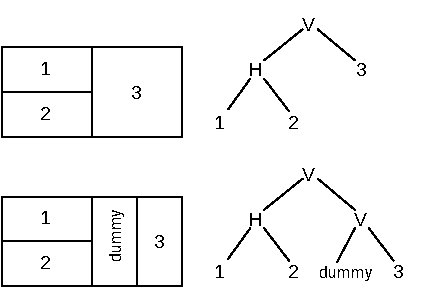
\includegraphics[height=0.33\textheight, center]{dummy_painting}
    \caption[Example of dummy painting injection]{Example of dummy painting injection to guarantee the free space between paintings 1,2 and 3.}
    \label{fig:dummy-painting}
\end{figure}

\subsection{Non-rectangular layouts}\label{subsec:non-rectangular-layouts}

Another extension to the proposed solution is adding the ability to work with layouts that are not rectangular.
It can be solved using the dummy paintings described in subsection~\ref{subsec:free-space}.
These dummy paintings must be created as small as possible and placed over the parts of the layout that are not rectangular.
By placing such created dummy facilities, the layout becomes rectangular.
A similar approach is used in~\cite{scholzExtensionsSTaTSPractical2010} to modify a slicing tree to solve FLP (sec.~\ref{sec:facility-layout-problem}).

An example of using dummy paintings to work with a non-rectangular layout is in figure~\ref{fig:non-rectangular-layout}.
There are two irregularities in both corners of the layout.
Two dummy paintings are injected into the slicing tree to fill the irregularities.

\begin{figure}[h!]
    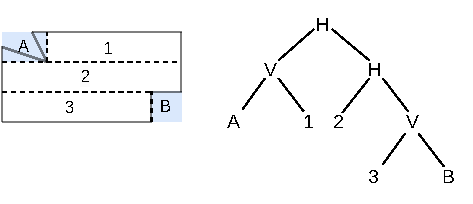
\includegraphics[width=0.8\textwidth, center]{non-rectangular-layout}
    \caption[Example of working with non-rectangular layout]{Example of working with non-rectangular layout. The allocated area is marked using a dotted line.
    Dummy paintings that fill the irregularities in both corners are A and B.}
    \label{fig:non-rectangular-layout}
\end{figure}

\subsection{Non-rectangular paintings}\label{subsec:non-rectangular-paintings}

Another extension is to allow painting shapes that are not rectangular.
This problem can be easily solved by representing a non-rectangular painting
as the smallest possible rectangle to which the painting fits.
By using this approach, the proposed implementation can work with non-rectangular paintings.
One possible drawback is that the painting placement solution might become more sparse,
i.e., containing too much free space.
However, this can be solved using a post-optimization heuristic that tries to reduce a free space
of a painting placement solution.

\subsection{Placing heuristic}\label{subsec:placing-heuristic}

Instead of using the placement heuristic described in subsection~\ref{subsec:placement-heuristic}, a different one can be used.
One candidate is a heuristic that, instead of trying to place painting in the corners of the allocated area,
tries to place the painting at all possible placement points, e.g., to place the painting in the middle of the allocated area.
However, using this solution might be computationally expensive.
On the other hand, a heuristic that only tries the bottom-left of the allocated area as a placement point can be much faster but
might not produce good results.

Another approach is calculating suboptimal or optimal placement points inside the allocated area.
Then, move the painting as close as possible to that point.
A similar approach is used in~\cite{goncalvesBiasedRandomkeyGenetic2015} for solving FLP (sec.~\ref{sec:facility-layout-problem}).
They move the facility centroid as close as possible to the calculated unconstrained optimum without leaving the
boundaries where the facility can be placed.

\subsection{Post-optimization}\label{subsec:post-optimization}

One interesting idea is to introduce post-optimization.
It is a process that takes the result, in this case, the painting placement solution,
and tries to improve it.
For example, if there is insufficient free space between paintings, they can be moved by the post-optimization process.
Another example will be if the goal is to create the most compact layout.
Then, a solution can be to use the compaction operation proposed in~\cite{laiSlicingTreeComplete2001},
which tries to reduce free space as much as possible.

\subsection{Extension to other problems}\label{subsec:extension-to-other-problems}

The solution proposed in this method can be applied to other problems.
The central part of the thesis is the coding of an individual and crossover.
These can be used to solve problems that optimize some permutation of elements.

One concrete example is 2D-KP problem with rectangular pieces~\cite{bortfeldtGeneticAlgorithmTwodimensional2009},
where the objective is to place as many rectangles in a container as possible,
minimizing unused space.
The solution proposed in this thesis can solve the 2D-KP problem with rectangular pieces by
using unchanged individual representation (sec.~\ref{sec:coding}), unchanged decoding procedure (subsec.~\ref{subsec:individual-decoding}),
and unchanged slicing layout construction (subsec.~\ref{subsec:slicing-tree-construction}).
Then, the problem-specific placement heuristic places the rectangles,
followed by BL heuristic~\cite{chazelleBottomnLeftBinPackingHeuristic1983} that minimized unused space.

\subsection{Deciding which painting to place}\label{subsec:deciding-which-painting-to-place}
Deciding which painting to place can happen when the wall area is insufficient to place all paintings.
Thus, some subset of paintings has to be selected and placed.
A similar problem is solved in the shelf-space planning problem (sec.~\ref{sec:shelf-space-planning}),
where the retailer has to decide which goods to place on shelves to achieve maximum profits.

\subsection{Multiple walls}\label{subsec:multiple-walls-for-painting-placement}

The painting placement problem can be extended to contain multiple walls instead of one.
Additionally, the walls might have some interactions between them, e.g., placing a painting on the first wall
limits the subset of paintings that can be placed on the second wall.
A similar problem is solved in the shelf-space planning problem (sec.~\ref{sec:shelf-space-planning}),
where there are multiple shelves at the same time.

\subsection{Human operator assistance}\label{subsec:human-operator-assistance}
Painting placement solution, which is some placement of paintings, can be easily visualized.
Thus, it can be presented to a human operator that will further modify it.

For example, FLP (sec.~\ref{sec:facility-layout-problem}) creates a layout for multiple facilities.
A human engineer that creates the plan for placing these facilities might use the output of an algorithm as a starting point.
Then, the engineer can modify it by increasing the aisle size or changing the position of some facilities.
